\documentclass{article}
\usepackage{tikz}
\usepackage[utf8]{inputenc}
\usepackage[spanish]{babel}
\usepackage{graphicx}
\usepackage{hyperref}
\usepackage{amsmath}
\usepackage{geometry}
\usepackage{fancyhdr}
\usepackage{enumitem}
\usepackage{tcolorbox}
\usepackage{amssymb}
\usepackage{pgfplots}
\usepackage{pgfplotstable}
\usepackage{pgfplots}
\pgfplotsset{compat=1.18}
\usepackage{pgf-pie} % Paquete para gráficos de pastel
\usepackage{multicol}
\usepackage{array}
\usepackage{booktabs}
\usepackage{xcolor}
\usepackage{booktabs}
\usepackage{array}
\geometry{margin=1in}
\usepackage{multirow}
\usepackage{tikz}
\usetikzlibrary{shapes, positioning, arrows.meta}
\usepackage{amsmath}
\usepackage{colortbl}
\usepackage{xcolor}
\usepackage{tcolorbox} % Paquete para cuadros de texto
\usepackage{tikz}
\usetikzlibrary{shapes, positioning}

% Color a los links
\hypersetup{
    colorlinks=true,
    linkcolor=blue, % Color de los enlaces internos
    urlcolor=red    % Color de los enlaces externos
}

% Configuración de márgenes
\geometry{top=3cm, bottom=2
cm, left=2.5cm, right=2.5cm}

% Configuración del encabezado y pie de página
\pagestyle{fancy}
\fancyhf{}
\fancyhead[L]{\textbf{Universidad Politécnica de Valencia - UPV}}
\fancyhead[R]{\thepage}
\rfoot{
\includegraphics[scale=0.03]{Logo_Iberdrola_(2023).svg.png}}
\fancyfoot[C]{}
\fancyfoot[L]{\textbf{Dirección e innovación estratégica.}}



% Título del documento
\title{ \textbf{Dirección e innovación estratégica.\\} Trabajo final}
\author{Satorre J, García F y Gracia J}
\date{Noviembre 17 de 2024}

\begin{document}
\thispagestyle{empty}

% Portada
\maketitle
\begin{center}
    
\includegraphics[width=0.5\textwidth]{Logo_Iberdrola_(2023).svg.png} \\ % agregar un logo aquí
    
\end{center}
\rule{\linewidth}{0.2mm}
\begin{center}
    
\includegraphics[width=0.45\textwidth]{UPV-Emblem.png} \\ 
\end{center}
\rule{\linewidth}{0.2mm}
% Crear la caja de resumen
\begin{tcolorbox}[colback=yellow!15!white, colframe=green!30!black, title=\textbf{Resumen}]
El mapa del recorrido del comprador de Iberdrola muestra que procesos como comprar o usar el producto es muy fácil para el comprador. 
\\

También presenta unos importantes retos para el comprador en términos de inversiones, sobre para los clientes institucionales dado que el producto producido y comercializado por Iberdrola no se utiliza de manera directa. 
\\

En cuanto a los no clientes, Iberdrola tiene potencial para atraer a los no clientes de segundo nivel. Debe trabajar de manera intensa y coherente con el fin de construir relaciones de largo plazo, basadas en la confianza, con estos potenciales compradores. 
\\
\dotfill
\\

\textbf{Palabras clave: Mapa del comprador, niveles de no clientes, océano azul, seis caminos} 
\end{tcolorbox}

\newpage

% Índice
\tableofcontents
\newpage
\listoffigures
\newpage
\listoftables
\newpage

% Introducción
\section{Introducción}
Este documento examina la estrategia de Iberdrola en el contexto del mercado energético español, centrándose en su enfoque de dirección e innovación estratégica. La estrategia de Iberdrola se dirige a consolidar su posición en un mercado cada vez más competitivo, caracterizado por cambios en las preferencias del consumidor, el aumento de la competencia y una creciente demanda de energías renovables. Dentro de este contexto, el análisis aborda tres temas clave: el mapa de utilidad del comprador, la segmentación de los niveles de no clientes y las posibles estrategias de captación para estos grupos.
\\

En el mapa de utilidad del comprador, se estudian las distintas etapas que atraviesa el consumidor en su interacción con los servicios de Iberdrola y cómo estos se adaptan para maximizar la satisfacción y la experiencia del usuario. Aspectos como el acceso a la energía, la facilidad de uso y el valor percibido de los servicios son fundamentales para mejorar la percepción de los consumidores sobre Iberdrola y destacar su propuesta de valor frente a otros proveedores de energía en el mercado.
\\

Por otra parte, el documento introduce los niveles de no clientes como una herramienta de segmentación clave que permite identificar a aquellos individuos o grupos que no forman parte del mercado actual de Iberdrola, pero que tienen el potencial de integrarse en él bajo las condiciones adecuadas. Esta segmentación divide a los no clientes en tres niveles: el primer nivel incluye a quienes consideran cambiar a Iberdrola, pero aún no han dado el paso; el segundo nivel agrupa a consumidores que prefieren otros proveedores, generalmente locales, por cercanía o personalización; y el tercer nivel se centra en comunidades rurales o aisladas que carecen de acceso a la red eléctrica convencional.
\\

Finalmente, se presentan estrategias de captación orientadas a atraer a cada uno de estos segmentos. Estas estrategias sugieren iniciativas de personalización, ofertas de beneficios tangibles y construcción de confianza como medios para captar clientes que, por distintos motivos, no han considerado a Iberdrola como una opción viable. En conjunto, estos enfoques buscan fortalecer la posición de Iberdrola en el mercado y facilitar su expansión a nuevos segmentos, fomentando una percepción positiva y de valor en clientes actuales y potenciales.
\newpage
\section{Unidades de negocio de Iberdrola.}
La generación y comercialización de energía eléctrica compite en el sector energético, específicamente en el subsector eléctrico. 

\begin{figure}[h!]
    \centering
    \caption{\textbf{Gráfico PMC para las unidades de negocio de Iberdrola. Fuente: Iberdrola. Elaboración propia.}}
    \label{fig:enter-label}

\begin{tikzpicture}

% Define colors for each level
\definecolor{colono}{RGB}{4,164,72}
\definecolor{migrante}{RGB}{255,157,19}
\definecolor{pionero}{RGB}{4,171,255}

% Draw the main rectangular box
\draw[thick] (0,0) rectangle (13,9);

% Draw horizontal dividers
\draw[thick] (0,3) -- (13,3);
\draw[thick] (0,6) -- (13,6);

% Add labels for each level
\node[anchor=east, text=blue!60!white] at (-0.5,7.5) {\textbf{PIONERO}};
\node[anchor=east, text=blue!50!white] at (-0.5,6.5) {Innovación en valor};
\node[anchor=east, text=orange] at (-0.5,4.5) {\textbf{MIGRANTE}};
\node[anchor=east, text=orange] at (-0.5,3.5) {Mejora de valor};
\node[anchor=east, text=green!70!black] at (-0.5,1.5) {\textbf{COLONO}};
\node[anchor=east, text=green!70!black] at (-0.5,0.5) {Imitación de valor};

% Plot bubbles for each data point with respective size and color

% Nivel Colono
\fill[colono] (3,1.8) circle (1); 
\node[anchor=north] at (3,0.9) {\footnotesize Generación y Comercialización de energía};

\fill[colono] (7,2.1) circle (0.8); 
\node[anchor=north] at (7,1.4) {\footnotesize Redes eléctricas};

\fill[colono] (7,0.5) circle (0.1); 
\node[anchor=north] at (7,0.4) {\footnotesize Transporte de energía};

% Nivel Migrante
\fill[migrante] (2.5,4) circle (0.2); 
\node[anchor=west] at (2.7,4) {\footnotesize Autoconsumo y energía distribuida};

\fill[migrante] (6.5,5.5) circle (0.2); 
\node[anchor=west] at (6.7,5.5) {\footnotesize Soluciones de eficiencia energética};

% Nivel Pionero
\fill[pionero] (1,7.5) circle (0.2); 
\node[anchor=west] at (1.2,7.5) {\footnotesize Soluciones energéticas y servicios personalizados};

\fill[pionero] (5.5,8.5) circle (0.15); 
\node[anchor=west] at (5.7,8.5) {\footnotesize Movilidad eléctrica};

\fill[pionero] (4.5,8) circle (0.12); 
\node[anchor=west] at (4.7,8) {\footnotesize Hidrógeno verde};

% Add legend
\draw[thick] (9,1) circle (0.5) node[right=0.5cm] {Ingresos cuantiosos};
\draw[thick] (9,2) circle (0.2) node[right=0.5cm] {Ingresos reducidos};

\end{tikzpicture}
\end{figure}

\subsection{Principales unidades de negocios.}
 
 \begin{enumerate}
     \item \textbf{Generación y Comercialización de energía:} dividido en dos sectores, que son energías renovables (eólica terrestre y marina, energía solar, hidroeléctrica) y generación convencional y comercialización
    \item \textbf{Redes eléctricas:} incluye el mantenimiento y la operación de las infraestructuras eléctricas que transportan la energía desde los generadores hasta el consumidor final.
    \item \textbf{Transporte de energía:} a través de grandes líneas de alta tensión.
    \item \textbf{Soluciones energéticas y servicios personalizados:} gravamos con grandes proyectos y nos ajustamos a los requerimientos del cliente para ayudarle a solucionar su problema o necesidad. 
    \item \textbf{Autoconsumo y energía distribuida:} Promueven el autoconsumo mediante la instalación de placas solares en empresas y hogares.
    \item \textbf{Soluciones de eficiencia energética:} ayuda a los clientes a reducir el consumo energético a través de la instalación de energías más eficientes.
    \item \textbf{Movilidad eléctrica:} Instala puntos de recarga para vehículos eléctricos.
    \item \textbf{Hidrógeno verde:} Clave para la descarbonización de los sectores más difíciles de electrificar, como por ejemplo el transporte de larga distancia. Se obtiene utilizando electricidad generada a través de fuentes renovables.
 
 \end{enumerate}
\subsection{Datos de las dos grandes unidades de negocio de Iberdrola.}

En la figura 1 se observa la distribución de las unidades e negocio de Iberdrola dentro del gráfico de PMC. 
\\

En el cuadro siguiente vemos los ingresos de las dos unidades de negocio más grandes y el resto de unidades aparecen como otros. 
\\

Se aprecia que la Generación de energía y comercialización es la unidad de negocio con mayores ingresos para la empresa con, aproximadamente 30 mil millones de euros para 2023. Esto representa un 63\% de los ingresos. 
\\
Le sigue redes con cerca de 18 mil millones de euros y representa un 36\% de los ingresos.
\\
Por último, muy lejos están los ingresos por otras líneas de negocio con 44 millones de euros y con una participación de cerca al 0.1\%. 

\begin{table}[h!]
    \centering
    \resizebox{1\textwidth}{!}{ % Cambia 0.8 para ajustar el tamaño a un 80% del ancho de la página
    \begin{tabular}{|l|c|c|c|c|}
        \hline
        \textbf{Negocios} & \textbf{2020} & \textbf{2021} & \textbf{2022} & \textbf{2023} \\
        \hline
        Redes (M Eur) & 12.900 € & 14.887 € & 18.355 € & 18.363 € \\
        Producción de Electricidad y Clientes (M Eur) & 20.692 € & 24.777 € & 36.294 € & 31.683 € \\
        Otros Negocios (M Eur) & 107 € & 60 € & 42 € & 44 € \\
        \hline
        \textbf{Ingresos Totales} & \textbf{33.698 €} & \textbf{39.724 €} & \textbf{54.692 €} & \textbf{50.091 €} \\
        \hline
        Redes (\%) & 38,3\% & 37,5\% & 33,6\% & 36,7\% \\
        Producción de Electricidad y Clientes (\%) & 61,4\% & 62,4\% & 66,4\% & 63,3\% \\
        Otros Negocios (\%) & 0,32\% & 0,15\% & 0,08\% & 0,09\% \\
        \hline
    \end{tabular}}
    \caption{Ingresos de Iberdrola por unidad de negocio en millones de euros y participación porcentual. Fuente: Iberdrola. Elaboración propia.}
    \label{tab:ingresos_iberdrola}
\end{table}

\section{Descripción y selección de la unidad de negocio.}
Para el presente estudio se selecciona la unidad de negocio \textit{"Generación y comercialización de energía"}. 
\\
Los sectores al que pertenece la actividad de generación y comercialización de energía son: 
\begin{itemize}
    \item \textbf{Sector industrial.} Este sector abarca la producción y generación de energía. Aquí se incluye toda la infraestructura y actividad relacionada con la transformación de recursos naturales como el gas, petróleo, carbón, viento y radiación solar en energía utilizable. Las empresas que operan plantas de generación (hidroeléctricas, nucleares, solares, eólicas, etc.) se clasifican en esta categoría.
    \item \textbf{Sector servicios.} La comercialización y distribución de energía se considera parte del sector de servicios. Este sector incluye actividades relacionadas con la venta de energía a consumidores residenciales, industriales, comerciales; y servicios asociados, como el mantenimiento de redes, facturación, atención al cliente y la gestión de contratos.
\end{itemize}

\subsection{Principales empresas en España que tienen unidades de negocio de generación y comercialización de energía.}
En el cuadro 2 se mencionan las principales empresas que tienen unidades de negocio de generación y comercialización de energía. 
\\

\begin{table}[h]
    \centering
    \begin{tabular}{|p{4cm}|p{11cm}|}
        \hline
        \textbf{Empresa}                                      & \textbf{Descripción}                                                                                                                                           \\ \hline
        Iberdrola                                    & Una de las mayores empresas energéticas de España, que opera en la generación de electricidad a partir de diversas fuentes, incluyendo energías renovables.    \\ \hline
        Endesa                                       & Filial de Enel, es una de las principales compañías de generación y comercialización de electricidad y gas en España.                                           \\ \hline
        Naturgy                                      & Ofrece servicios de generación de electricidad y gas, con un enfoque en la sostenibilidad y las energías renovables.                                           \\ \hline
        Acciona Energía                              & Especializada en energías renovables, dedicada a la generación de electricidad a partir de fuentes como la eólica, solar y biomasa.                           \\ \hline
        EDP Renewables                               & Parte del grupo EDP, se enfoca en la generación de energía a partir de fuentes renovables, incluyendo eólica y solar.                                          \\ \hline
        Repsol                                       & Conocida tradicionalmente como una compañía de petróleo y gas, ha estado invirtiendo en energías renovables y en la generación de electricidad.                   \\ \hline
        Grup Energía de Barcelona (GEB)             & Centrada en la generación y comercialización de electricidad, especialmente a través de fuentes renovables.                                                     \\ \hline
        Fenie Energía                                & Se dedica a la comercialización de energía eléctrica y a la promoción de soluciones energéticas.                                                                  \\ \hline
        Holaluz                                      & Comercializadora de electricidad enfocada en ofrecer energía 100\% renovable a sus clientes.                                                                      \\ \hline
        Energía Solar de Castilla y León (Escyl)    & Especializada en la generación de energía solar fotovoltaica.                                                                                                   \\ \hline
    \end{tabular}
    \caption{Empresas que tienen unidades de negocio de generan y comercializan energía en España. Elaboración propia.}
    \label{tab:energia}
\end{table}


\section{Proceso de estratégico para la unidad de negocio.}
\subsection{Técnica de \textit{Speed Thinking}}
Se utilizó la técnica de \href{https://upvedues-my.sharepoint.com/:b:/g/personal/jjgralop_upv_edu_es/EWA5ZRDOYpNIp2X1rahk_8IBIYG8gKvQJj9uIZHmW4Mf-Q?e=OrpQcz}{Speed Thiking} para determinar los factores que pueden afectar al sector de la generación y distribución de energía según los integrantes del equipo. 
\\

En el cuadro 3 se observan los factores mencionados por cada persona del equipo. 
\\
Factores como la sostenibilidad, eficiencia, Precio, fiabilidad, Almacenamiento, fueron mencionados por varios integrantes del equipo. 
\begin{table}[h]
    \centering
    \begin{tabular}{|p{5cm}|c|c|c|}
        \hline
        \textbf{Factores} & \textbf{Jhon Gracia} & \textbf{Jorge Satorre} & \textbf{Fernando García} \\ \hline
        Calidad           &                     & X                      & X                         \\ \hline
        Experiencia       &                      &                    & X                         \\ \hline
        Solidez           &                      &                       & X                         \\ \hline
        Sostenibilidad    & X                    & X                      & X                        \\ \hline
        Eficiencia        & X                    &                        & X                        \\ \hline
        Global            &                      &                       &   X                       \\ \hline
        Innovación        &                      &                      &  X                        \\ \hline
        Adaptabilidad     &                      &                    &  X                        \\ \hline
        Diversificación   &                      &                   &  X                        \\ \hline
        Precio            & X                    & X                      &                          \\ \hline
        Cadena de suministro & & X              &                          \\ \hline
        Atención al cliente & & X               &                          \\ \hline
        Almacenamiento    & X                    &  X                     &                          \\ \hline
        Inversión en tecnología & & X           &                          \\ \hline
        Cumplimiento normativo & & X            &                         \\ \hline
        Fiabilidad        & X                    & X                      &                          \\ \hline
        Generación estable & X                  &                        &                          \\ \hline
        Variabilidad de producción & X          &                        &                          \\ \hline
        Manejo del mix de producción & X        &                        &                          \\ \hline
        Flexibilidad de suministro & X          &                        &                          \\ \hline
    \end{tabular}
    \caption{Tabla de factores por cada persona del equipo. Elaboración propia.}
    \label{tab:factores}
\end{table}

\subsection{Factores comunes para al análisis de la unidades de negocio.}

Para realizar el escenario estratégico debemos elegir varios factores clave sobre los que compite el sector, y seleccionar con quién nos vamos a comparar. 
Para el presente análisis se compara la unidad de Generación y distribución de energía de Iberdrola con las unidades de negocio de dos empresas fuertes del sector ubicadas en España: Endesa y Naturgy.

\subsection{Factores clave del equipo en la generación y distribución de energía.}
\begin{enumerate}
    \item \textbf{Precio:} Es un factor crucial para los consumidores, especialmente en el sector de energía donde las tarifas afectan tanto a los hogares como a las industrias. Las empresas que logran mantener precios competitivos pueden atraer y retener a más clientes. 
    \item \textbf{Calidad:} Se refiere a la consistencia y estabilidad del suministro energético. Los consumidores y empresas dependen de una energía que no tenga interrupciones. 

    \item \textbf{Fiabilidad:} Está directamente relacionada con la calidad del suministro y la capacidad de la empresa para responder ante eventualidades, como picos de demanda o interrupciones en la red. 
    \item \textbf{Sostenibilidad:} Ha ganado gran relevancia en el sector energético, impulsada por la creciente preocupación por el cambio climático y las regulaciones ambientales. Las empresas que generan energía limpia (solar, eólica, hidroeléctrica) y que reducen sus emisiones de carbono son preferidas tanto por clientes conscientes como por los gobiernos.

    \item \textbf{Distribución:} La distribución de energía implica la infraestructura necesaria para llevar la electricidad o el gas hasta el cliente final. La expansión de la red de distribución en áreas rurales o remotas es un aspecto diferenciador que permite captar nuevos mercados.

    \item \textbf{Innovación:} La innovación es clave en el sector energético, con avances en generación renovable, almacenamiento, redes inteligentes, y gestión de la demanda. 

    \item \textbf{Cumplimiento normativo:} El sector energético está altamente regulado, y las empresas deben cumplir con normativas ambientales, de seguridad y de competencia.

    \item \textbf{Almacenamiento:} La capacidad de almacenamiento de energía es un aspecto diferenciador clave, especialmente en energías renovables como la solar y la eólica, que dependen de condiciones climáticas variables. Las empresas que invierten en almacenamiento, como baterías de larga duración o almacenamiento de hidrógeno, pueden garantizar un suministro más estable y aprovechar mejor su capacidad de generación.

    \item \textbf{Variabilidad del producto:} La variabilidad del producto en el sector energético implica ofrecer diferentes tipos de energía o servicios a los clientes, como tarifas de energía verde, energía de respaldo o planes personalizados según el consumo. 

\end{enumerate}
\subsection{Calificación de los factores para cada unidad de negocio de Iberdrola y los dos competidores.}
\begin{table}[h]
    \centering
    \caption{Puntuación de los factores de las unidades e negocio de generación y distribución de energía de Iberdrola y competidores. Elaboración propia.}
    \begin{tabular}{|p{5cm}|c|c|c|}
        \hline
        \textbf{Factores} & \textbf{Iberdrola} & \textbf{Naturgy} & \textbf{Endesa} \\ \hline
        Precio           &   4                  & 3                      & 3                         \\ \hline
        Calidad       &     4                 &     3               & 4                        \\ \hline
        Fiabilidad           &    5                  &     5                 & 5                         \\ \hline
        Sostenibilidad    & 5                    & 5                      & 4                        \\ \hline
        Distribución        & 4                    & 3                       & 4                        \\ \hline
        Innovación            &  3                    &  4                     &   3                       \\ \hline
        Cumplimiento normativo        &   5                   & 5                     &  5                        \\ \hline
        Almacenamiento     &  5                    &  3                  &  4                        \\ \hline
        Producción variable   &  5                    &  2                 &  2                        \\ \hline
    \end{tabular}
    \label{tab:factores}
\end{table}

\subsection{Gráfica y análisis de los resultados.}
En la figura 2 se observa el comportamiento de las unidades de negocio de las empresas competidoras en azul y rojo y de Iberdrola en color verde. 
\\

En cuanto al factor precio, la calidad, sostenibilidad, distribución, innovación Almacenamiento, Variabilidad de la producción Iberdrola presenta una calificación más alta.
\begin{figure}[h!]
    \centering
    \begin{tikzpicture}
        \begin{axis}[
            xlabel={},
            xtick={1,2,...,9},
            xticklabels={Precio, Calidad, Fiabilidad, Sotenibilidad, Distribución, Innovación, Cumplimiento normativo, Almacenamiento, Producción variable},
            xticklabel style={rotate=30, anchor=east},
            ytick=\empty, % Esta línea elimina los números en el eje Y
            legend pos=north west,
            width=1.1\textwidth,
            height=0.6\textwidth
        ]
        \addplot [color=green!50!black, line width=2pt] coordinates {(1,4.1) (2,4.2) (3,4.6) (4,4.7) (5,3.9) (6,4.3) (7,4.8) (8,5) (9,4.8)};
        \addlegendentry{Iberdrola}
        \addplot [color= blue, line width=1.5pt] coordinates {(1,3.3) (2,3.1) (3,4.6) (4,3.9) (5,3.8) (6,3.7) (7,4.8) (8,3.5) (9,3.4)};
        \addlegendentry{Naturgy}
        \addplot [color=red, line width=1.5pt] coordinates {(1,2.9) (2,3.7) (3,4.8) (4,3.8) (5,3.7) (6,3.4) (7,4.8) (8,3.4) (9,3.6)};
        \addlegendentry{Endesa}
        \end{axis}
    \end{tikzpicture}
    \caption{Gráfico de lineas que compara los factores entre Iberdrola, Naturgy y Endesa. Elaboración propia.}
    \label{fig:comparacion}
\end{figure}

Por otro lado, en temas de fiabilidad está igual a Naturgy y es superado por Endesa. Por último, en el cumplimiento normativo, las tres unidades de negocio están iguales. 





\section{Mapa de utilidad del comprador de energía de Iberdrola.}
La figura 1 muestra el mapa del comprador de energía de Iberdrola, en función de las seis etapas del ciclo de la experiencia del comprador de energía y las seis palancas de utilidad que se usan en general para la construcción de la matriz. 
\begin{figure}[h!]  % [h] significa aquí (justo en el lugar donde aparece el código)
    \centering
    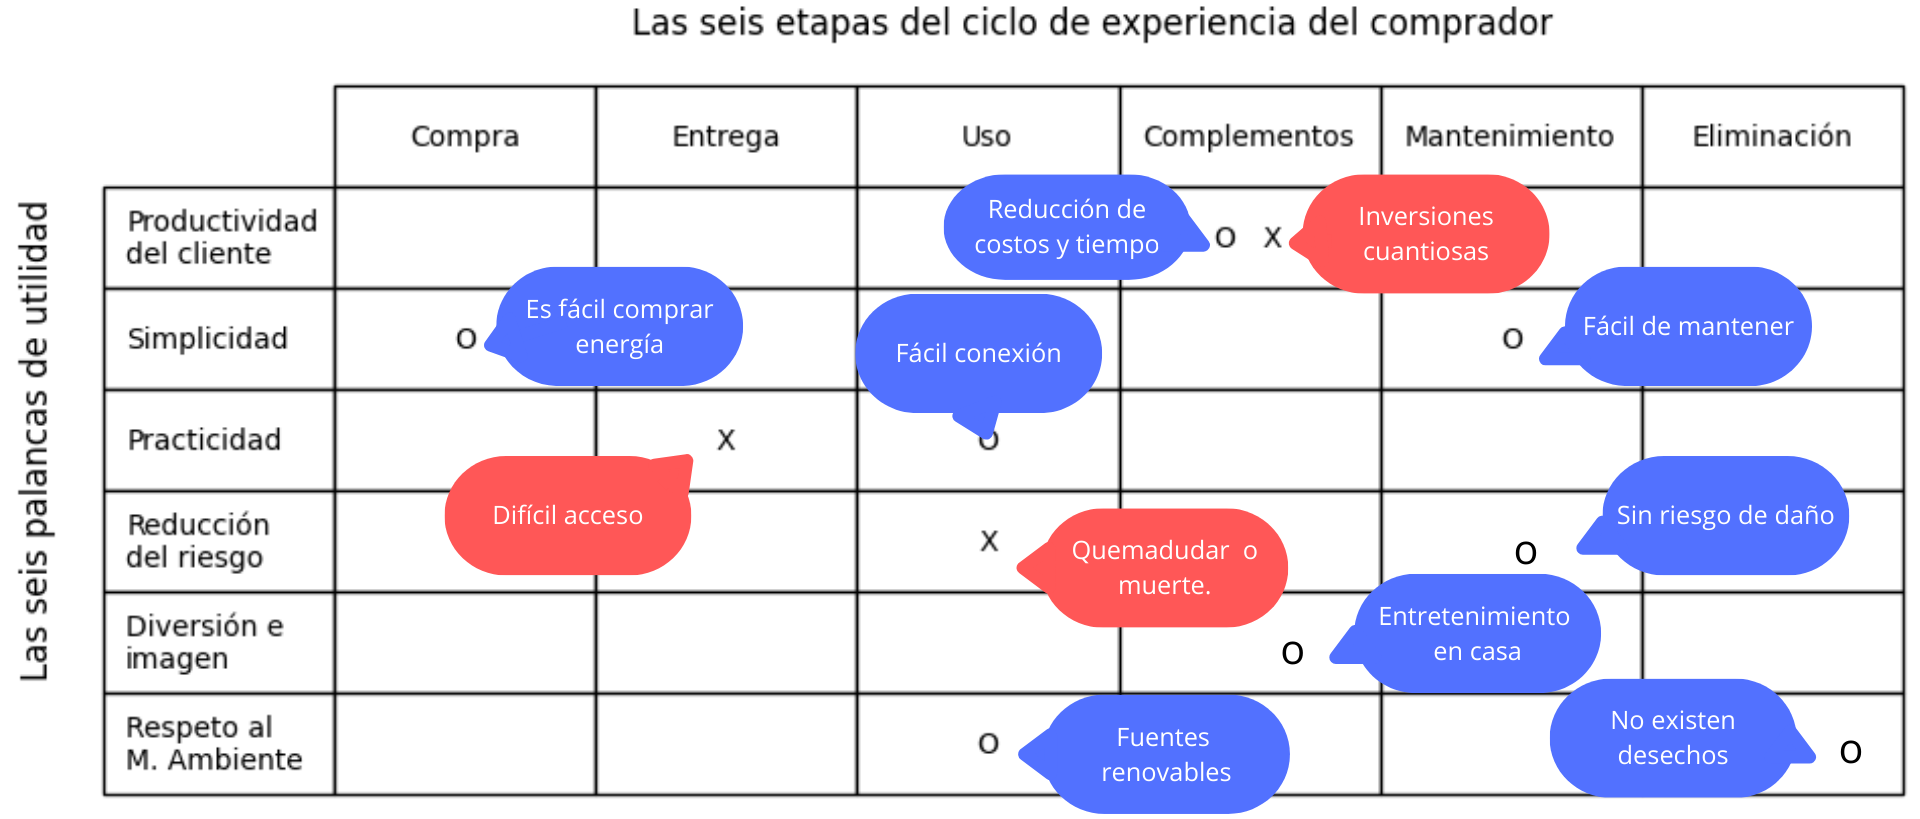
\includegraphics[width=1\textwidth]{Mapa de utilidad.png}  % Ajusta el tamaño y nombre del archivo
    \caption{Mapa de utilidad del consumidor de energía de Iberdrola. Elaboración propia.}
    \label{fig:mi_imagen}
\end{figure}

\begin{itemize}
    \item Se observa que la compra de energía es un proceso fácil de realizar para el comprador. La empresa Iberdrola cuenta con un excelente equipo de ventas, con profundos conocimientos técnicos sobre el producto. También cuenta con canales de ventas presencial y online. 
    \item En algunas ocasiones existe una infraestructura de transmisión de electricidad deficiente y en otros casos inexistente, por tanto para el comprador de energía puede ser difícil el acceso o imposible. 
    \item Iberdrola ofrece al comprador la oportunidad de consumir energía de fuentes renovables en su mayor proporción. 
    \item El producto que produce y comercializa Iberdrola es peligroso para el comprador, dado que una incorrecta manipulación puede causar daños graves o la muerte. 
    \\
    La empresa toma todos los controles necesarios y suficientes, legales, técnicos, sociales, económicos para brindar al cliente un producto con un muy reducido riesgo para el comprador. 
    \item El uso de la energía que produce y comercializa Iberdrola es de fácil uso para el comprador. Sólo requiere conexión a la instalación al interior del hogar, empresa, oficina, etc. 
    \item La energía como producto no transmite su valor de manera directa, por razones que los inherentes a su naturaleza; sino que opera como un insumo para dispositivos en general. 
    \\
    Entonces, es a través de estos dispositivos que transmite su valor y genera productividad más alta que otras fuentes de energía, en muchos casos generando una mayor rendimiento o desempeño.   
    \\

    La parte negativa es que en muchas ocasiones se requiere de grandes inversiones en dispositivos para aprovechar el poder de la energía eléctrica. Inversiones en dispositivos eléctricos que son más costosos que sus análogos que operan con otras fuentes de energía como el carbón, diesel, gasolina, etc. 
    \item Las instalaciones eléctricas dentro de la empresa, hogar, oficina., no son, en geneal, complejas, por tanto son fáciles de mantener para el comprador.  
    
\end{itemize}
\section{Niveles de no clientes para la empresa Iberdrola.}
Los niveles de no clientes son una forma de segmentar a aquellos que no forman parte del mercado actual de una empresa pero que tienen el potencial de serlo. Se clasifican en tres niveles, según su proximidad al mercado existente. 

\begin{figure}[h!]
\centering
\begin{tikzpicture}

% Dibujar el cuadro (rectángulo)
\draw[thick] (-1,-4) rectangle (14,4);  % Cuadro alrededor de los círculos

% Colocar texto dentro del rectángulo
\node at (6, 3.5) {};  % Texto dentro del rectángulo

% Dibujar los círculos y colocar texto dentro de cada uno
\draw[fill=blue!50] (1,0) circle (2cm);   % Círculo pequeño
\node[align=center] at (1, 0) {\textbf{No clientes.} \\ \textbf{ Primer nivel.} \\ Usan la conexión \\ a la red eléctrica, \\ sólo si es preciso.};  % Texto en el primer círculo

\draw[fill=orange!50] (6.5,-0.5) circle (3.5cm);   % Círculo mediano
\node[align=center] at (6.5,-0.5) {\textbf{No clientes. Segundo nivel.} \\ Usan otras \\ fuentes de energía. \\ Tienen acceso a la red, pero \\ no quieren hacer uso de esta.};  % Texto en el segundo círculo

\draw[fill=green!50] (12,0) circle (2cm);  % Círculo grande
\node[align=center] at (12, 0) {\textbf{No clientes.}\\ \textbf{Tercer nivel.}\\No usan energía. \\ No se han conectado \\ porque \\ no tienen acceso.};  % Texto en el tercer círculo

\end{tikzpicture}
\caption{Tres niveles de no clientes para la empresa Iberdrola. Elaboración propia.}
\end{figure}

\begin{itemize}
    \item \textbf{Primer nivel de no clientes:} Son personas que se encuentran cerca del mercado actual y están considerando entrar, pero aún no lo han hecho debido a barreras como precio, accesibilidad, percepción del valor, etc. 
    \\
    
    Estos son consumidores que están considerando cambiar su proveedor de energía a Iberdrola, pero aún no han dado el paso. \\
    Por ejemplo podrían ser hogares o empresas que están insatisfechos con su actual proveedor, ya sea por precios altos, mal servicio al cliente o falta de compromiso con la sostenibilidad, y ven en Iberdrola una alternativa viable o clientes actuales de otras compañías energéticas que se sienten atraídos por las ofertas de Iberdrola en energías renovables o tarifas competitivas. 
    \item \textbf{Segundo nivel de no clientes:} Son aquellos que conocen el mercado o el producto, pero lo rechazan activamente. Pueden considerar que la oferta actual no se adapta a sus necesidades o que no vale la pena el esfuerzo o coste involucrado.
    \\
    
    Aquí se encuentran aquellos que, por alguna razón, conocen Iberdrola pero no han optado por sus servicios. Por ejemplo serían consumidores que prefieren proveedores locales más pequeños por cercanía o percepción de mayor personalización, usuarios que desconfían de las grandes empresas energéticas o que tienen una mala experiencia previa con compañías similares y hogares o negocios que consideran que las tarifas verdes (energías renovables) son más caras o que no les ofrecen un beneficio tangible.
    \item \textbf{Tercer nivel de no clientes:}Son personas que nunca han sido consideradas como posibles clientes, ya sea porque no están familiarizadas con el producto o servicio o porque la industria no los ve como una oportunidad viable.
    \\
    
    Estos son individuos o grupos que nunca han sido considerados como clientes potenciales para Iberdrola, a menudo porque no están conectados con el mercado energético convencional.  Por ejemplo serían comunidades rurales o aisladas que no tienen acceso a la red eléctrica tradicional y dependen de fuentes alternativas como generadores de diésel o energía solar, consumidores en mercados emergentes que aún no están conectados a servicios de electricidad centralizados y personas o empresas que consideran generar toda su energía de manera autosuficiente (por ejemplo, con paneles solares y baterías) y no ven necesidad de conectarse a un proveedor como Iberdrola.
    \end{itemize}
\section{Estrategia para intentar captar a cada uno de
estos grupos.}
En este caso se ha decidido por las personas que se encuentran en el segundo nivel, ya que el objetivo de esta estrategia es tratar de cambiar su rechazo hacía la compañía por una que les haga cambiar la visión que tienen sobre Iberdrola. \\
Para el segundo nivel la estrategia elegida sería basada en la personalización, confianza y beneficios tangibles.
Con la propuesta de personalización sería a través del diseño de tarifas o planes que permitan a los clientes elegir según la opción que les sea más conveniente, un ejemplo sería el crear tarifas con tramos más bajos.
Con la propuesta de beneficios tangibles sería a través de la posibilidad de comunicar el ahorro a largo plazo que pueden tener los clientes al elegir energías renovables o también el ofrecerles descuentos temporales o instalaciones gratuitas para la primera vez. \\
Con la propuesta de confianza sería a través de simplificar las condiciones que hay en los contratos y eliminar las cláusulas ocultas para reducir su desconfianza hacia la empresa o poner ejemplos de clientes reales que con el cambio a esta compañía hayan visto mejorado su situación.

\section{Ejecuta tu jugada}
En la feria del océano azul se presenta el mapa de utilidad del consumidor de energía de Iberdrola, que aparece en la figura 3 del presente documento, también se presentan los tres niveles de no clientes de Iberdrola que parece en la figura 4 del presente documento. 
\\

Se presenta el escenario estratégico inicial con los valores de cada uno de los factores de la unidad de negocio para las tres empresas: Iberdrola, Endesa y Naturgy. 
\\

A partir de aquí se desarrollan los seis caminos para reorientar las fronteras del sector de la producción y comercialización de energía eléctrica.
\\

Los seis caminos son una herramienta que nos permite generar posibles nuevos factores que redefinan la unidad de negocio. El primer camino es la exploración de sectores alternativos. Se exploran los sectores de energía fósil, los cuales, por sus características tienen factores de producción, almacenamiento y comercialización diferentes al sector de energía eléctrica. El segundo camino es la exploración de los grupos estratégicos del sector de la energía eléctrica. Se toma como referencia algunos factores de la generación de energía de manera descentralizada. Para el tercer el tercer camino se busca explorar la cadena de compradores brindando la oportunidad al comprador de gestionar las redes de consumo de energía a través de la creación de redes inteligentes. El cuarto camino explora son los factores que inciden en los servicios complementarios de la producción y la comercialización de energía eléctrica como las plataformas de optimización de la producción de energía y el almacenamiento descentralizado en manos del cliente. El quinto camino es la orientación de la unidad de negocio hacia los funcional y emocional. Los nuevos factores son la igualdad de acceso a la energía que afecta emocionalmente al consumidor  y las dificultades que las personas tienen con el cambio tecnológico. Por último, se explora el futuro para tratar de incluir nuevos factores que son y serán tendencia. En la generación y comercialización de energía, la tendencia gira hacia un mayor consumo de energía de fuentes renovables que va atada a la necesidad del aumento de la producción de energía. 
\\

Se realiza la exposición de cada uno de los seis caminos planteados. Cada camino contiene una matriz ERIC y un escenario estratégico proyectado. 
\\

El escenario seleccionado es el segundo camino con el factor de producción de energía portable combinado con dos factores del primer camino en base a los factores de almacenamiento potencial y generación de energía \textit{in situ.} 
\\

La matriz ERIC final, resultado del la feria del océano azul es la siguiente: 
\begin{figure}[h!]
    \centering
    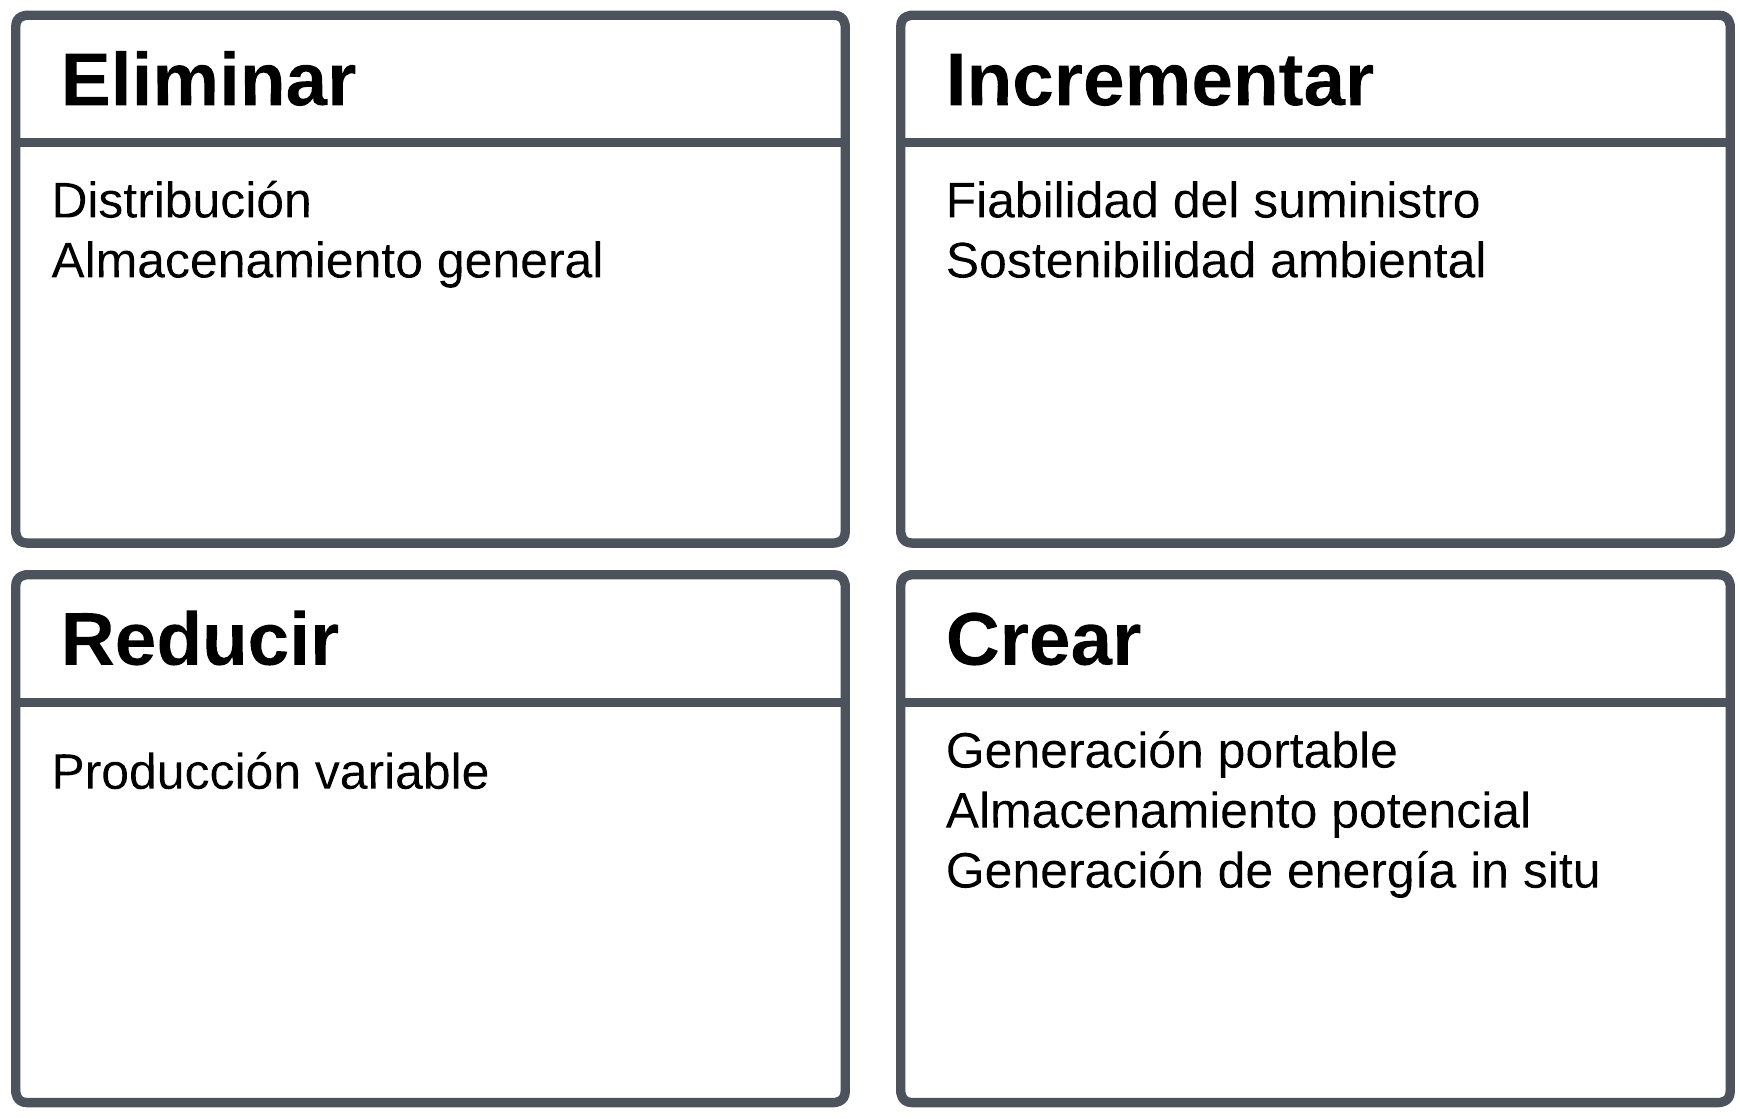
\includegraphics[width=0.8\linewidth]{Matriz eric.png}
    \caption{\textbf{Matriz ERIC resultado de la feria del óceano azul.}}
    \label{fig:enter-label}
\end{figure}

En la figura 5 se aprecia la matriz ERIC que agrega tres factores nuevos al sector de la generación y distribución de energía eléctrica: 
\begin{itemize}
    \item \textbf{Generación portable.} Generar energía con equipos de menos tamaño al actual en los lugares donde se requiere. 
    \item \textbf{Almacenamiento potencial.} Tomar los excesos de energía generada por fuentes variables y aprovecharla para subir agua hacia las presas que tiene la empresa. 
    \item \textbf{Generación de energía \textit{in situ}.} Generar energía en el mismo lugar donde se produce la fuente de dicha generación. 
\end{itemize}

\begin{figure}[h!]
    \centering
    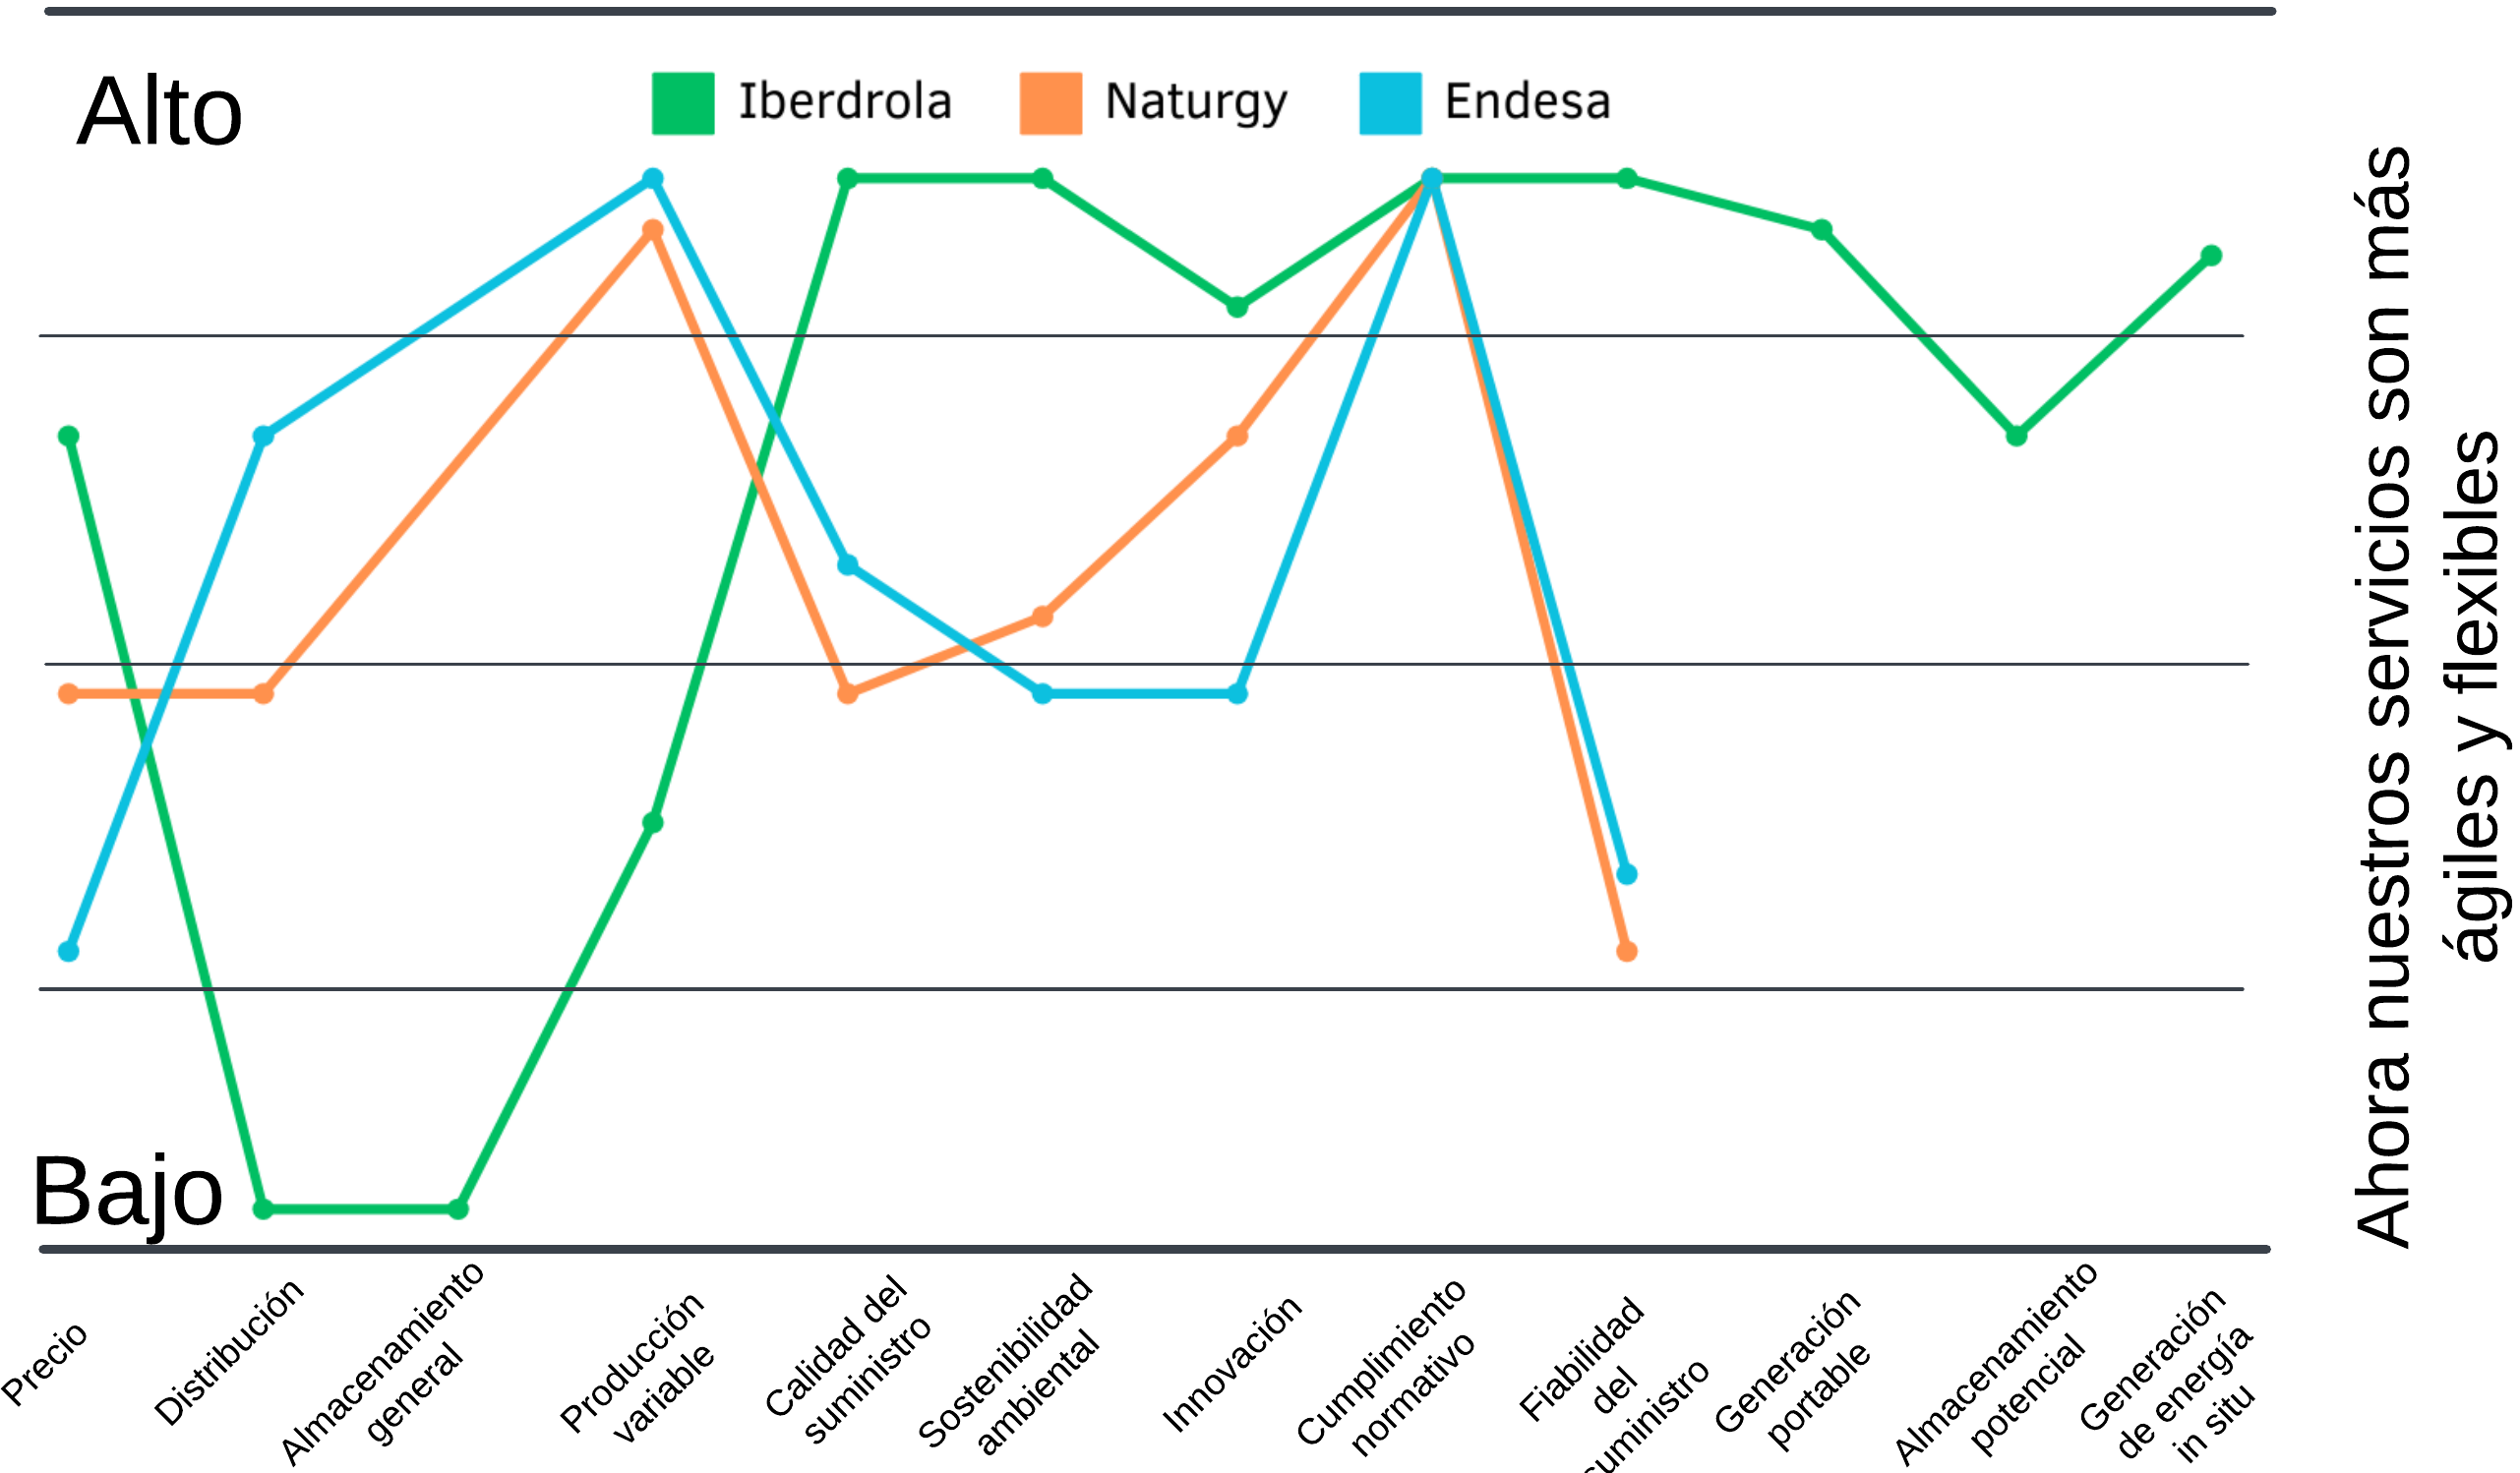
\includegraphics[width=0.8\linewidth]{Estrategico futuro.png}
    \caption{\textbf{Escenario estratégico proyectado con los nuevos factores.}}
    \label{fig:enter-label}
\end{figure}

Al la derecha de la figura 6 se aprecia la linea verde que representa los nuevos factores que se integran a la unidad de negocio de generación y comercialización de energía. Genera un nuevo foco que permite a la unidad de negocio diferenciarse de la competencia.  

\section{Cambios en el mapa de utilidad del consumidor} 
Al integrar los nuevos factores a la unidad de negocio de generación y comercialización de energía eléctrica, se modifica el mapa de utilidad del consumidor de energía. Las mejoras en la utilidad del comprador son:
\begin{itemize}
    \item \textbf{Fiabilidad del suministro.} La entrega de energía eléctrica se vuelve más fiable hacia las grandes empresas que requieren una cantidad de energía constante. Esto se debe a que la generación portable de energía se realiza cerca de las empresas que requieren el suministro. La generación y la comercialización se produce casi de manera personalizada. 
    \item \textbf{Suministro más sostenible.} El almacenamiento potencial, es decir, como agua en una presa, permite aumentar la generación de energías renovables las cuales son de producción variable, porque se puede almacenar para su uso futuro, reduciendo así la necesidad de producción de energías con combustibles fósiles.
    \item \textbf{Cambiar de tipo de energía.} Con la generación portable muchas empresas pueden cambiarse a una nueva forma de energía con la operan en sus procesos. Por ejemplo: Pueden pasar del uso del gas para calentar líquidos a calentarlos con energía eléctrica. 
\end{itemize}
Ahora, los dolores que se eliminar al comprador son: 
\begin{itemize}
    \item \textbf{Difícil acceso.} Con la generación de energía portable, el comprador ahora tiene acceso a energía que se produce cerca de su consumidor. 
\end{itemize}
\begin{figure}[h!]
    \centering
    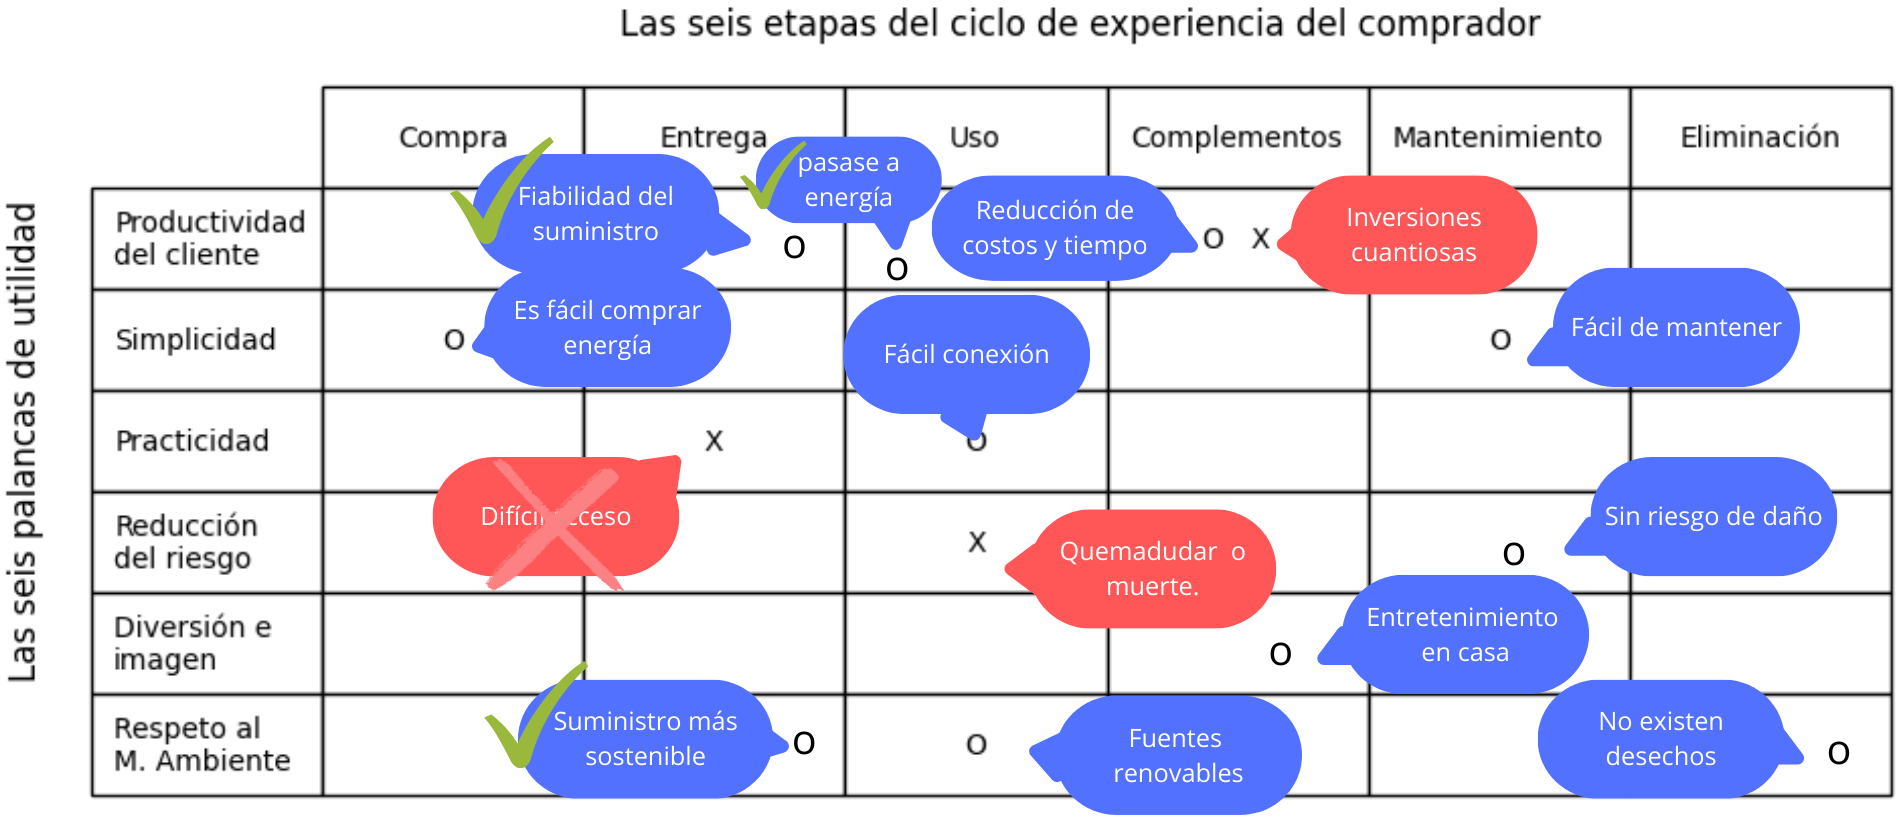
\includegraphics[width=1\linewidth]{mapa de utilidad.png}
    \caption{\textbf{Nuevo mapa de utilidad del comprador de energía eléctrica.}}
    \label{fig:enter-label}
\end{figure}
En la figura 7 se aprecia en azul como el modelo de negocio impacta de manera positiva sobre el comprador de energía eléctrica. En rojo se observan los puntos de dolor de algunos usuarios y no usuarios de la energía eléctrica suministrada por Iberdrola. El punto marcado con una X significa que ese punto de dolor se elimina con los nuevos factores que se integran al modelo de negocio. 
\\

Los punto azules con un \textit{check} de color verde son las nuevas utilidades que se generan para el comprador a partir de la integración de los nuevos factores. 
\section{Precios}
Energía Eléctrica:

El precio de la electricidad varía a lo largo del día según la demanda y la oferta. El precio medio de la luz hoy es de 0,1979 €/kWh. La hora más barata es de 03:00 a 04:00, con un precio de 0,1362 €/kWh, y la más cara de 19:00 a 20:00, con un precio de 0,3091 €/kWh. 

Gas Natural:

El precio del gas natural depende de la tarifa contratada y del consumo anual. Para un consumo anual entre 5.000 y 15.000 kWh (tarifa RL.2), los precios en el mercado regulado (TUR) son:

Término fijo: 5,66 €/mes
Término variable: 0,0565 €/kWh 
PRECIOGAS
En el mercado libre, las tarifas pueden variar. Por ejemplo, Repsol ofrece:

Término fijo: 10,90 €/mes
Término variable: 0,0599 €/kWh 


\begin{figure}[h!]
    \centering
    \label{fig:enter-label}

\begin{tikzpicture}

% Define colors for each level
\definecolor{colono}{RGB}{155,155,155}
\definecolor{migrante}{RGB}{155,155,155}
\definecolor{pionero}{RGB}{155,155,155}

% Draw the main rectangular box
\draw[thick] (0,0) rectangle (11,9);

% Draw horizontal dividers
\draw[thick] (0,3) -- (15,3);
\draw[thick] (0,6) -- (15,6);
\draw[thick] (15,6) -- (15,3);
\draw[thick] (11,4) -- (15,4);
\draw[thick] (11,5) -- (15,5);

% Add labels for each level

\node[anchor=north, text=black] at (9,10) {Gas natural};

\node[anchor=north, text=black] at (2,10) {Energía eléctrica};


% Plot bubbles for each data point with respective size and color

% Nivel Colono
\fill[colono] (2,1.8) circle (0.2); 
\node[anchor=north] at (2,1.7) {\footnotesize 0.12€ kw/h};

\fill[colono] (9,1.1) circle (0.2); 
\node[anchor=north] at (9,1.9) {\footnotesize 0.05€ kw/h};


% Nivel Migrante
\fill[migrante] (2,4.2) circle (0.9); 
\node[anchor=south] at (2,5) {\footnotesize Entre 0.15€ y 0.23€ kw/h};

\fill[migrante] (9,4.3) circle (1.2); 
\node[anchor=south] at (9,5.4) {\footnotesize Entre 0.08€ y 0.24€ kw/h};

% Nivel Pionero
\fill[pionero] (2,7.5) circle (0.2); 
\node[anchor=south] at (2,7.6) {\footnotesize 0.30 € kw/h};

\fill[pionero] (9,8.5) circle (0.15); 
\node[anchor=south] at (9,7.7) {\footnotesize 0.35€ kw/h};

\fill[migrante] (2,4.2) circle (0.1); 
\node[anchor=south] at (2,5) {\footnotesize Entre 0.15€ y 0.23€ kw/h};

% Límites 
\fill[migrante] (15,6) circle (0.05); 
\node[anchor=west] at (15,6) {\footnotesize 0.25€ kw/h};

\fill[migrante] (15,3) circle (0.05); 
\node[anchor=west] at (15,3) {\footnotesize 0.07€ kw/h};

\fill[migrante] (15,5) circle (0.05); 
\node[anchor=west] at (15,5) {\footnotesize 0.19€ kw/h};

\fill[migrante] (15,4) circle (0.05); 
\node[anchor=west] at (15,4) {\footnotesize 0.13€ kw/h};

\end{tikzpicture}
  \caption{\textbf{Bandas de precios del gruso del mercado de la energía.}}
\end{figure}


\section{Costes}
\section{Adopción}
\section{Modelo de negocio}

\section{Reflexiones.}
El análisis del mapa de utilidad del comprador muestra que, si bien Iberdrola ofrece un proceso de compra sencillo y múltiples canales de acceso, existen desafíos relacionados con el acceso de algunas comunidades y generar confianza en consumidores que actualmente utilizan otras fuentes de energía.
\\

La identificación de los niveles de no clientes es crucial para el crecimiento de Iberdrola. Al reconocer segmentos como aquellos que prefieren proveedores locales o comunidades sin acceso a la red eléctrica, se subraya la necesidad de que la empresa adapte sus estrategias para ofrecer soluciones personalizadas que respondan a las preferencias de estos grupos y así ganarse su confianza.
\\

La estrategia de captación de clientes basada en personalización, beneficios tangibles y construcción de confianza es fundamental para cambiar la percepción de Iberdrola entre los consumidores escépticos. Implementar tarifas flexibles, simplificar contratos y proporcionar ejemplos de casos de éxito ayudaría a fortalecer la reputación de la empresa y atraer a nuevos clientes, aumentando su competitividad en el mercado.
\newpage

% Bibliografía
\newpage
\section{Bibliografía}
\begin{thebibliography}{9}
\bibitem{}
Iberdrola. (2024). Plan Online de luz: Ofertas y tarifas. Recuperado el 15 de noviembre de 2024, de https://www.iberdrola.es/luz/ofertas-plan-online?utm\_source=google\&utm\_medium=cpc\&utm\_content=2216586129\&utm\_campaign=2011/Search/
Brand/Exact\&utm\_term=iberdrola\&wtarget=kwd-1124983116\&wcmp=62353089\&gad\_source=1\&gclid=
Cj0KCQi
A\_9u5BhCUARIsABbMSPstSqMLBWC7v-kzaiJkk6tewYa3NhTjk1Ty5n2TJmdZGdaGqVsClq
0aAp4CEALw\_wcB\&gclsrc=aw.ds
\bibitem{}
Iberdrola. (2024). Iberdrola: Energía y soluciones para tu hogar. Recuperado el 15 de noviembre de 2024, de https://www.iberdrola.es/
\bibitem{Iberdrola}
Iberdrola. (2024). Informe integrado ESG. Recuperado el 31 de octubre de 2024, de https://www.iberdrola.com/accionistas-inversores/informacion-operativa-financiera/informes-anuales/informe-integrado-esg/. 
\bibitem{Iberdrola}
Iberdrola. (2024). Nuestra actividad. Recuperado el 31 de octubre de 2024, de https://www.iberdrola.com/conocenos/nuestra-actividad. 
\bibitem{Iberdrola}
Iberdrola. (n.d.). Información operativa y financiera. Iberdrola. Recuperado el 2 de noviembre de 2024, de https://www.iberdrola.com/accionistas-inversores/informacion-operativa-financiera
\bibitem{}
Norvento. (2023). El sector energético en España. Recuperado el 2 de noviembre de 2024, de https://www.norvento.com/blog/el-sector-energetico-en-espana/
\bibitem{}
Ministerio para la Transición Ecológica y el Reto Demográfico. (2024). Sector eléctrico. Recuperado el 2 de noviembre de 2024, de https://www.miteco.gob.es/es/energia/energia-electrica/electricidad/sector-electrico.html
\bibitem{}
Statista. (2024). El sector energético en España. Recuperado el 2 de noviembre de 2024, de https://es.statista.com/temas/7651/el-sector-energetico-en-espana/

\bibitem{}
Tarifas Gas Luz. (2025). Comparador de precios del gas. Recuperado el 12 de enero de 2025, de https://tarifasgasluz.com/comparador/precio-kwh-gas



\end{thebibliography}
\end{document}
